In this section, the results from previous sections will be compared with those in an ANSYS Mechanical finite element analysis (FEA) software \cite{ANSYS}. Please note that all results presented in the foregoing section will utilize USC units. Important results will be converted to their respective SI units.

\section{Model}

Using the $D_o , L$ parameters from Table~\ref{table:prelim_params}, the drum geometry was modeled as a thin surface to save computational cost and time. The geometry and coordinate system adopted in this preceding analysis are shown below in Figure~\ref{fig:4_geom}.

\begin{figure}[H]
	\centering
	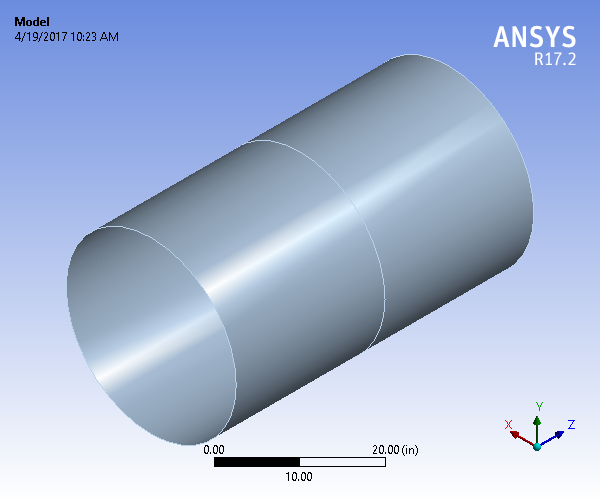
\includegraphics[scale=0.5]{4_geom}
	\caption{Geometry and coordinate system overview.}
	\label{fig:4_geom}
\end{figure}

In this model, the drum's thin surface has a parameterized inward thickness. Parametric studies will be performed in ANSYS with this variable to see how maximum stress and deformation vary. The thin surface also allows for a simply initial coarse mesh generated in ANSYS (see Figure~\ref{fig:4_mesh}).

\begin{figure}[H]
	\centering
	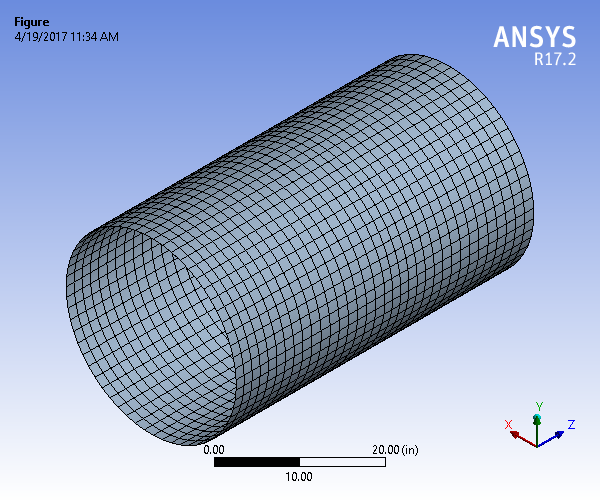
\includegraphics[scale=0.5]{4_mesh}
	\caption{ANSYS generated coarse mesh.}
	\label{fig:4_mesh}
\end{figure}

To assure numerically accurate results, a mesh refinement study will be performed on both maximum total deformation and equivalent (Von-Misses) stress for all foregoing simulations.

\section{Run 2}

The second run continues on the results determined from Run 1. The results presented in this foregoing section will focus on a barrel thickness of $0.50\ in$ 

\subsection{Boundary Conditions}

Both of the drum's ends are simply supported (i.e. BCs as per \ref{eq:2_endBC} ). In other words, simple supports carry no end moments.\\

Figure~\ref{fig:4_R2_tens} shows the location of applied tether tension of $11,525\ lbs.$ or $51,264\ N$.
\begin{figure}[H]
	\centering
	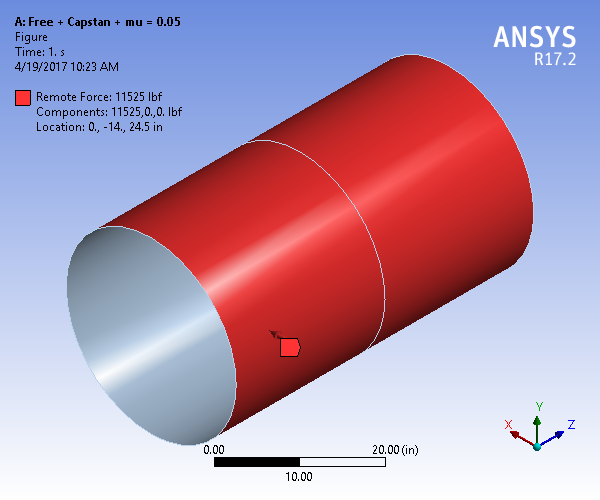
\includegraphics[scale=0.5]{4_R2_tens}
	\caption{Remote force location in ANSYS model.}
	\label{fig:4_R2_tens}
\end{figure}

Figure~\ref{fig:4_R2_pvar} shows the variable Capstan pressure applied as per results from \ref{subsection:alt} (see Figure~\ref{fig:4_R2_pvarplot} for $p(z)$ ). Note again that the boundary conditions are for $\mu=0.05$ , which is essentially the worst case scenario.

\begin{figure}[H]
	\centering
	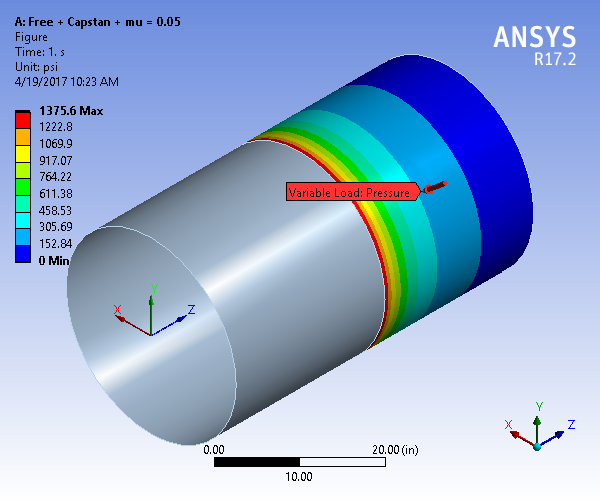
\includegraphics[scale=0.5]{4_R2_pvar}
	\caption{Variable Capstan pressure.}
	\label{fig:4_R2_pvar}
\end{figure}
\begin{figure}[H]
	\centering
	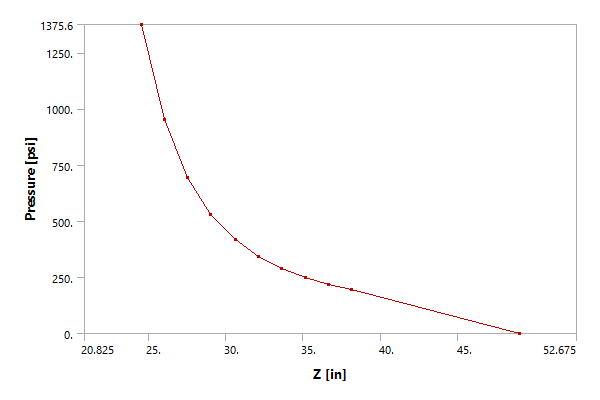
\includegraphics[scale=0.6]{4_R2_pvarplot}
	\caption{Variable Capstan pressure as a function of longitudinal coordinate $z$.}
	\label{fig:4_R2_pvarplot}
\end{figure}


\subsection{Results}

After a mesh refinement, total deformation results are shown below in Figure~\ref{fig:4_R2_def_mu05}. The maximum deformation seen on the top surface of the drum in the $y$ direction with respect to $z$ are also shown in Figure~\ref{fig:4_R2_topdefplotmu05}.

\begin{figure}[H]
	\centering
	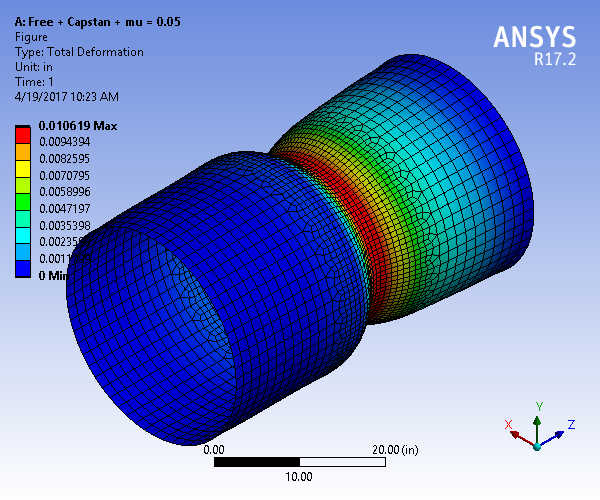
\includegraphics[scale=0.5]{4_R2_def_mu05}
	\caption{Total deformation results.}
	\label{fig:4_R2_def_mu05}
\end{figure}
\begin{figure}[H]
	\centering
	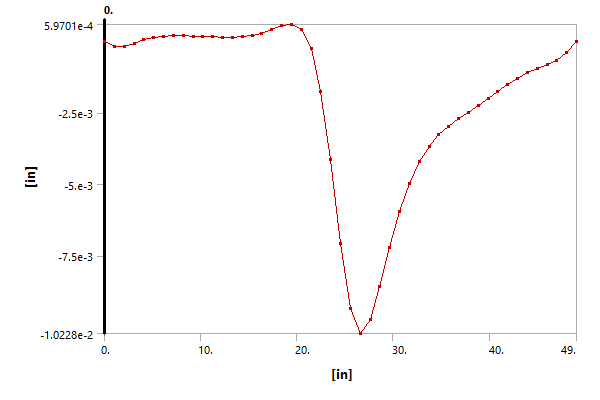
\includegraphics[scale=0.6]{4_R2_topdefplotmu05}
	\caption{Total deformation in $y$ as a function of $z$.}
	\label{fig:4_R2_topdefplotmu05}
\end{figure}

Comments, lots of deformation.\\

Again, post mesh refinement yields the maximum stress results as per Figure~\ref{fig:4_R2_stress_mu05}.

\begin{figure}[H]
	\centering
	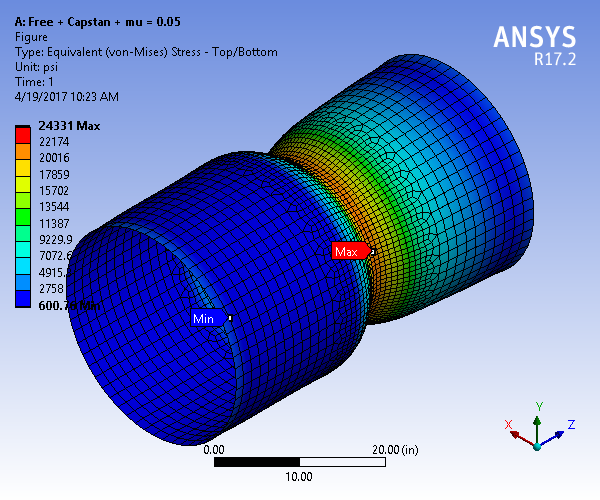
\includegraphics[scale=0.5]{4_R2_stress_mu05}
	\caption{Total stress results.}
	\label{fig:4_R2_stress_mu05}
\end{figure}

Comments, bad stress.


\subsection{Parametric Study}

A parametric study was ran with $0.15 \leq t \leq 1.05$ and $0.05 \leq \mu \leq 0.50$. This sweep results are shown below in Figure~\ref{fig:4_R2_sweep} \cite{EXCEL}. The allowable stress limit of $\sigma_{allow}=\sigma_{y}/SF = 23,333\ psi$ is also shown for reference.

\begin{figure}[H]
	\centering
	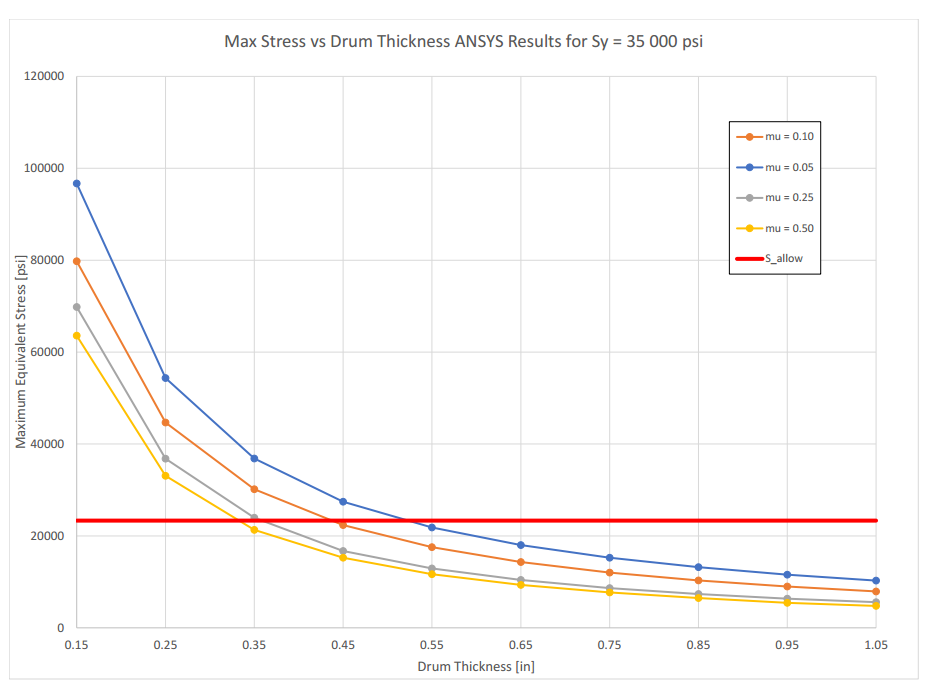
\includegraphics[scale=0.6]{4_R2_sweep}
	\caption{Results of parametric study for FEA Run 2.}
	\label{fig:4_R2_sweep}
\end{figure}

From the above plot, it appears as though a thickness of $t \geq 0.50\ in$ would appear to be sufficient.

